\documentclass[11pt]{article}

\usepackage[margin=1in]{geometry}
\usepackage{amsmath}
\usepackage{booktabs}
\usepackage{array}
\usepackage{graphicx}
\usepackage{float}
\usepackage{caption}
\usepackage[hidelinks]{hyperref}

\graphicspath{{../output/}{./}}   % ./ lets it compile in Overleaf with scenarios.png uploaded alongside
\setlength{\parskip}{0.5em}
\setlength{\parindent}{0pt}

\title{Canadian Macroeconomic Scenarios:\\ Oil Prices and US Growth, 2026Q3--2028Q3}
\author{Angel Gonzales}
\date{October 2026}

\begin{document}
\maketitle

\begin{abstract}
\noindent This report builds three scenarios for the Canadian economy over 2026Q3--2028Q3 and computes them into forecasts for real GDP, unemployment, CPI inflation, the Bank of Canada policy rate and new house prices. Using two exogenous variables that Canada does not control: the WTI oil price and US real GDP growth, 
I estimate a VAR, calibrated over the period 2009Q3 to 2026Q2, and forecast key Canadian macroeconomic variables using the paths of the exogenous variables. In the downside
scenario, a US slowdown with oil falling to \$50, calibrated to the 2001 US recession, Canadian GDP
contracts for three consecutive quarters, unemployment peaks near 7.9\%, and the policy rate falls close
to 0.25\% by mid-2028. All code and data are available at \url{https://github.com/Angelgonzales7067/Canada_macro_scenario}.
\end{abstract}

% -----------------------------------------------------------------------------
\section{Methodology}

\subsection{Data}

The sample is quarterly, 2009Q3 to 2026Q2 (68 quarters). It starts with the first full quarter of the
Bank of Canada's daily policy-rate series (V39079, available from April 21, 2009) and ends with the
latest quarter for which Canadian and US GDP are published. Monthly series are averaged to quarters
before transformation. Growth rates are computed as annualized log differences, $400\,\Delta\ln x_t$;
the oil price enters as the quarterly log change, $100\,\Delta\ln P_t$.

\begin{table}[htbp]
\centering
\caption{Variables, transformations and sources}
\small
\begin{tabular}{llll}
\toprule
Variable & Role & Form in model & Source \\
\midrule
WTI oil price           & Exogenous driver & $100\,\Delta\ln$, quarterly       & FRED, DCOILWTICO \\
US real GDP             & Exogenous driver & $400\,\Delta\ln$, annualized       & FRED, GDPC1 \\
Canada real GDP         & Endogenous       & $400\,\Delta\ln$, annualized       & StatCan 36-10-0104-01 \\
Unemployment rate       & Endogenous       & Level, \%                          & StatCan 14-10-0287-01 \\
CPI, all items (SA)     & Endogenous       & $400\,\Delta\ln$, annualized       & StatCan 18-10-0006-01 \\
Policy rate             & Endogenous       & Level, \%                          & Bank of Canada, V39079 \\
New Housing Price Index & Endogenous       & $400\,\Delta\ln$, annualized       & StatCan 18-10-0205-01 \\
\bottomrule
\end{tabular}
\end{table}

\subsection{Model}

The model is a VAR with exogenous variables (VARX):
\begin{equation}
  y_t = c + A_1\, y_{t-1} + B_0\, x_t + B_1\, x_{t-1} + \Gamma\, d_t + u_t ,
\end{equation}
where $y_t$ contains the five Canadian variables, $x_t$ contains oil-price growth and US GDP growth,
and $d_t$ contains dummy variables for 2020Q2 and 2020Q3 that absorb the COVID-19 collapse and rebound.
The choice of exogenous drivers is justified as Canada, as a small open economy, does not influence global oil prices or US growth. 

The lag length is one quarter because of limited observations. The model is estimated by OLS equation by equation using
the R package \texttt{vars}.

\subsection{Scenario forecasts and judgment}

For each scenario, the oil and US GDP paths are fed into the estimated model and the Canadian variables
are forecast nine quarters, conditional on those paths. The 2026Q3 oil price is set to its actual
average (\$87.12) in every scenario. For every scenario, the policy rate was imposed to be greater than or equal to 0.25\%

% -----------------------------------------------------------------------------
\section{Scenarios and historical calibration}

Each scenario's driver paths are calibrated to previous historical events to reflect real economic downturns (Table~\ref{tab:episodes})


\begin{table}[htbp]
\centering
\caption{Scenario assumptions, 2026Q3--2028Q3}
\label{tab:scenarios}
\small
\begin{tabular}{>{\raggedright\arraybackslash}p{1.8cm}>{\raggedright\arraybackslash}p{4.2cm}>{\raggedright\arraybackslash}p{1.9cm}>{\raggedright\arraybackslash}p{5.6cm}}
\toprule
Scenario & WTI path (US\$/bbl) & US real GDP & Historical calibration \\
\midrule
Baseline & Eases from \$87 to \$75 by 2027Q4, then flat & 2.0\% & US growth near potential and just below its 2010--19 average (2.4\% \\[0.3em]
Upside   & Drifts gently to \$70 by 2028Q3 & 3.0\% & 2017--19 expansion: US growth averaged about 2.8\%, WTI traded between \$48 and \$70 \\[0.3em]
Downside & Falls to \$68 in 2026Q4 and \$50 by 2027Q1, then flat ($-43\%$) & 0.5\% & 2001 US recession: US growth averaged 1.1\% over 2000Q3--2002Q4, WTI fell 36\%; the oil decline is similar to 1998 ($-44\%$) \\
\bottomrule
\end{tabular}
\end{table}

\begin{table}[htbp]
\centering
\caption{Historical episodes used for calibration (quarterly averages)}
\label{tab:episodes}
\small
\begin{tabular}{lcccc}
\toprule
Episode & WTI peak to trough & US growth & Canada GDP level & Canada unemp. \\
 & & (avg.) & (peak to trough) & (change) \\
\midrule
1998 Asia crisis      & \$23 $\to$ \$13 ($-44\%$)  & 4.4\%    & No decline   & No increase \\
2001 US recession     & \$32 $\to$ \$21 ($-36\%$)  & 1.1\%    & No decline   & $+1.0$ pt \\
2008--09 GFC          & \$124 $\to$ \$43 ($-65\%$) & $-0.3\%$ & $-4.4\%$     & $+2.5$ pts \\
2014--16 oil bust     & \$103 $\to$ \$33 ($-68\%$) & 2.7\%    & $-0.5\%$     & Flat (national) \\
\bottomrule
\end{tabular}

\vspace{0.3em}
\footnotesize Source: author's calculations from FRED and Statistics Canada data in the repository.
\end{table}

In this exercise, due to the simplicity of the model, I calibrated the downside scenario to a moderate contraction, rather than a severe recession.

% -----------------------------------------------------------------------------
\section{Results}

Table 4 reports 2027 averages and the gap from the baseline; Figure 1
shows the full quarterly paths.

\begin{table}[htbp]
\centering
\caption{2027 averages by scenario (growth rates annualized, \%)}
\label{tab:results}
\small
\setlength{\tabcolsep}{4pt}
\begin{tabular}{lrrrrrrr}
\toprule
 & WTI (\$) & US GDP & Canada GDP & Unemp. & CPI & Policy rate & House prices \\
\midrule
Baseline              & 78.4  & 2.0  & 1.44  & 7.11 & 1.29 & 1.80 & 0.12 \\
Upside                & 79.6  & 3.0  & 1.80  & 6.96 & 1.29 & 1.96 & $-0.05$ \\
Downside              & 50.0  & 0.5  & 0.15  & 7.58 & 0.42 & 1.39 & $-0.74$ \\
\midrule
Upside $-$ baseline   & 1.3   & 1.0  & 0.37  & $-0.15$ & 0.00 & 0.16 & $-0.17$ \\
Downside $-$ baseline & $-28.4$ & $-1.5$ & $-1.29$ & 0.47 & $-0.87$ & $-0.41$ & $-0.86$ \\
\bottomrule
\end{tabular}
\end{table}

\begin{figure}[H]
\centering
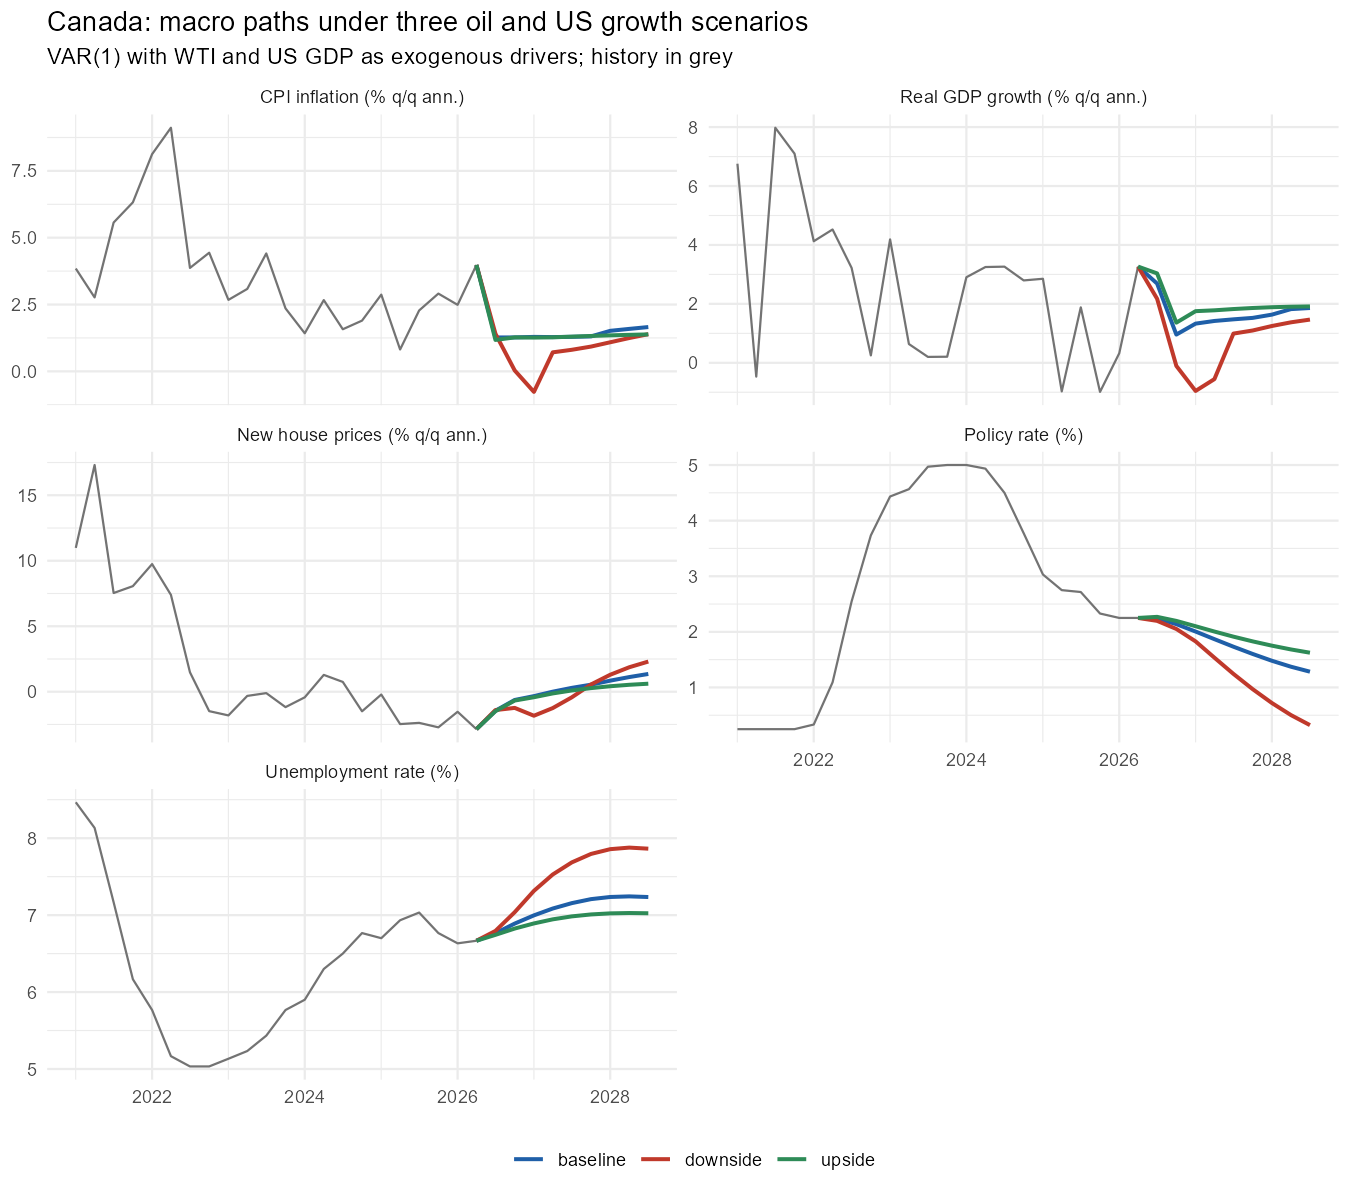
\includegraphics[width=\textwidth]{scenarios.png}
\caption{Canadian macro paths under the three scenarios}
\label{fig:paths}
\end{figure}

\textbf{Baseline.} The baseline scenario, which reflects market consensus paths for the key drivers, results in an initial decline in real GDP growth for Canada, followed by a rebound through 2027. CPI experiences a sharp decline as oil prices decrease, and then remains around target for the rest of the forecast, allowing flexibility for the central bank to cut rates through 2027. Unemployment ticks up past 7\%, and the housing price index goes up slightly.

\textbf{Downside.} Canadian real GDP contracts for three consecutive quarters (2026Q4--2027Q2), with the lowest level reaching $-1.0\%$ annualized in 2027Q1. This is a mild
technical recession, similar in severity to Canada's experience in 2001. Unemployment rises steadily to a
peak of about 7.9\% in 2028Q2, 1.2 points above its 2026Q2 level. Inflation goes below zero in
2027Q1 as lower oil prices cool down the economy, and the policy rate is cut to about 0.3\% by 2028Q. New house prices decline through 2027.

\textbf{Upside.} Stronger US demand lifts Canadian GDP growth by about 0.4 points relative to the baseline
in 2027, and unemployment is slightly lower. The policy rate remains slightly below 2026Q2 to support growth as inflation stays under control and housing prices rebound slightly.


% -----------------------------------------------------------------------------
\section{Limitations}

\begin{itemize}
  \item \textbf{Linearity.} The VAR model may not capture non-linear relationships or extreme responses to severe scenarios. Further work could include the use of Machine Learning for better prediction.
  \item \textbf{Short sample and imprecise estimates.} The policy-rate series limits the sample to
        68 quarters. As a result, some of the estimates may not be statistically significant.
  \item \textbf{Mean reversion.} With a relatively low number of observations, forecasting several quarters may produce estimates that drift toward the historical averages.
  \item \textbf{Missing channels.} For simplicity, some macroeconomic variables were omitted, which may produce omitted variable bias. These variables could include the Canada-US exchange rate, the Fed decisions, Canadian and US yields, etc.
  \item \textbf{Lack of structure} A structural VAR could be implemented to better simulate real-world conditions, where monetary and fiscal policy react to changes in macroeconomic variables at different times.
\end{itemize}

% -----------------------------------------------------------------------------
\section{AI Disclaimer}

AI was used in this project to assist with coding. Commentary is the Author's.

\end{document}
